\documentclass [11pt,fleqn]{article}

\usepackage{amssymb}
%\usepackage{epsf,psfig,graphicx}
\usepackage{epsf,graphicx}
\usepackage{psfrag}
\usepackage{amsmath}
\usepackage{color}
\topmargin     -0.60in  % (adjusted for printer bias) 
\headheight      .00in  % (no headers) 
\headsep         .50in  % (top margin + headers + skip) 
\textheight     9.50in  % (instructions: 9 1/8'' min, 9 7/16'' max) 
\textwidth      6.00in  % 2*3.33 + .33 = 6.99 
\oddsidemargin  0.3125in  % (subtracted 1inch bias) 
\evensidemargin 0.3125in 
%\renewcommand{\baselinestretch}{1.5} 
\parindent .0in 
\parskip 10pt 

\font \bigtenrm=cmmi10 scaled\magstep2 
\def \dt {\delta\tau} 
\def \ve {\varepsilon} 
\def \ch {{\cal H}} 
\def \del {\partial} 
\def \be {\begin{equation}} 
\def \ee {\end{equation}} 
\def \beq {\begin{eqnarray}} 
\def \eeq {\end{eqnarray}} 
\def \tv {\tilde v} 
\def \veren {\varepsilon^{\rm ren}_f} 
\def \vef {\varepsilon^0_f} 
\def \su {\uparrow} 
\def \sd {\downarrow} 
\def \CR {\nonumber\\} 
\def \hfb {\hfill\break} 
\def \tb {\bar{t} } 
\def \kb {\bar{k} } 
\def \tbB {\bar{t}_B } 
%\def \ul{#1} {$\underline{#1 }$}

\begin{document} 
\hspace{1cm}{\bf Title:} Observation of correlated x-ray scattering at atomic resolution \hfb
 
{\bf Authors:} Derek Mendez, Thomas J. Lane, Jongmin Sung,  Cl\`ement Levard, Herschel Watkins, Aina Cohen, Michael Soltis, Shirley Chisholm, James Spudich, Vijay Pande,  Daniel Ratner, Sebastian Doniach

{\bf Abstract}

Tools to study structure of disordered systems, such as proteins in solution, remain limited. Such understanding is essential for \emph{e.g.}~rational drug design. Correlated x-ray scattering (CXS) has recently attracted new interest as a way to leverage next-generation light sources to study such disordered matter. The CXS experiment measures the intensity correlation caused by the scattering of x-rays from an ensemble of identical particles, with disordered orientation and position. Averaging over 15,496 snapshot images obtained by exposing a sample of silver nanoparticles in solution to a micro-focused synchrotron beam, we report [ REMOVE ? for the first time REMOVE? ] an experimental CXS signal obtained from an ensemble in three dimensions. The correlation function was measured at  wide angles corresponding to atomic resolution and matches theoretical predictions. These results suggest that other CXS experiments on disordered ensembles -- such as proteins in solution -- may be possible in the future.


\section{Introduction}

In a pioneering paper, Kam \cite{Kam:1977wc} showed that correlated x-ray scattering (CXS) from an ensemble of randomly oriented particles could in principle reveal information about the internal structure of the particles beyond usual small and wide angle solution scattering measurements. The extraction of such information in the absence of an ordered system (\textit{e.g.}~a crystal) can be beneficial in biological studies, as many biological systems are inherently disordered (\textit{e.g.}~proteins in solution).

In order to gauge the feasibility of Kam's method at atomic length scales and to assess the associated difficulties, we conducted experiments measuring CXS from silver nanoparticle (NP) solutions at wide angles. Crucially, each measurement was conducted on an ensemble of NPs oriented randomly in three dimensions, extending previous work done in two dimensions \cite{Saldin:2011ch}, at small angles in 3-dimensions \cite{Kam:1981ua, Wochner:2009ia}, and on single particles in 3-dimensions \cite{Kam:1985tz, Starodub:1fy}. 

From these experiments, we obtained empirical correlation functions measuring the correlation between all pixel pairs in the first two silver Bragg rings. The three correlation functions (two rings with themselves, one between rings) show sharp peaks consistent with analytical and simulated predictions based on the crystal structure of silver. These peaks were deemed statistically significant by a Hotelling T-test [CITE] to a p-value of XXX [NEEEEEED THIS!].

By successfully measuring CXS signal from an ensemble of silver NPs, we have demonstrated the effectiveness of Kam's method given the current advances in x-ray technology. This experiment will serve as a benchmark for future experiments involving much weaker scatterers, such as proteins. It is our hope that the refinement of our our analysis techniques on a well known sample such as silver NPs will help facilitate the extension of CXS to studies of biomolecules in solution.

\section{Theory}

We briefly review the portions of \cite{Kam:1977wc} relevant to this manuscript. Let $S( \vec{q},\omega)$ represent the structure factor of an isolated particle in solution, i.e.

\be \label{structurefactor}
S(\vec{q},\omega) = \left| \> \int \rho \left(\hat{R} (\omega)\cdot \vec{r} \right) e^ { i \vec{q} \cdot \vec{r} } d\vec{r} \> \right| ^{2}
\ee
% electron density, not electronic -- TJL
where $\rho $ is the electron density throughout the particle volume, $\omega$ is a triple of Euler angles, and $\hat{R}(\omega)$ is a 3-dimensional rotation operator.

Kam showed that the correlation function

\be \label{correlation}
C(\vec{q}_1, \vec{q}_2) = \int S( \vec{q}_{1},\omega ) S( \vec{q}_{2},\omega ) \, d \omega %\,\, \equiv\,\, C(|\vec{q}_1|, |\vec{q}_2|,\psi)
\ee

may be extracted from a CXS measurement where one repeatedly records snapshots of a solution of $N$ identical particles, with each snapshot representing a unique ensemble of particles frozen in solution. Kam argued (assuming negligible inter-particle scattering interference) that the empirical correlation function averaged over shots would converge to (\ref{correlation}), \textit{i.e.},

\be \label{converge}
\langle \delta n_{s}(\vec{q}_1) \, \delta n_{s}(\vec{q}_2) \rangle_{s} \Rightarrow C(\vec{q}_1, \vec{q}_2) 
\ee

where $n_{s}(\vec{q})$ is the total photons scattered from all particles in snapshot $s \,\,(1 \leq s \leq N_{s} )$ into a pixel along momentum transfer vector $\vec{q}$ and $\delta n_{s}(\vec{q}) = n_{s}(\vec{q}) - \langle n_{s}(\vec{q}) \rangle_{s}$. Neglecting inter-particle scattering interference, $n_{s}(\vec{q})$ can be thought of as a linear combination of $S(\vec{q},\omega)$ for a set of orientations $\{ \omega\}_{s}$. We would like to emphasize that (\ref{correlation}) can be calculated using a model of $\rho$. This opens up the possibility for refining such a model against a CXS dataset using (\ref{converge}).

We have computed the expected correlation function (\ref{correlation}) for the silver NPs studied as a benchmark for our experimental results ( Figure 1 ) . A silver NP may be represented by a simple model consisting of a face-centered-cubic lattice cutoff by a spherical boundary. The scattering can then be represented by reciprocal lattice vectors cutting the Ewald sphere and giving rise to Bragg peaks broadened owing to the the finite size of the NPs.  Hence, each snapshot records a series of  Bragg rings. The sub-population of all NP orientations that simultaneously subtend two Bragg peaks on the Ewald sphere give rise to the correlations in (\ref{converge}). Let $\Delta$ be the angle between two scattering vectors $\vec{q}_{hkl}$ and $\vec{q}_{h'k'l'}$ satisfying the Bragg condition. Let $\phi$ be the azimuthal angle between the projections of $\vec{q}_{hkl}$ and $\vec{q}_{h'k'l'}$ into the plane perpendicular to an incident beam (corresponding to the angle between two pixels measuring $\vec{q}_{hkl}$ and $\vec{q}_{h'k'l'}$ on a farfield planar detector). Then

\be \label{angular}
C (|\vec{q}_{hkl}|,|\vec{q}_{h'k'l'}|, \Delta  ) = \left \langle \int_{0}^{2\pi} \delta n_{s} (| \vec{q}_{hkl}|,\phi ) \,\, \delta n_{s} (|\vec{q}_{h'k'l'}|,\phi + \Delta )\, d\phi  \right \rangle_{s}
\ee
% TJL thinks: HELPFUL!
is the average angular correlation of Bragg ring intensity fluctuations. One should expect CXS signal then at values of $\Delta $ corresponding to the geometry of the reciprocal lattice and the angles between reciprocal lattice vectors. For instance, $C (|\vec{q}_{111}|,|\vec{q}_{111}|, \Delta  )$ should display strong signal at $\Delta_1 = \arccos[ \frac{-2}{3\cos^{2}\theta} + 1  ]$ and $\Delta_2 = \arccos[ \frac{-4}{3\cos^{2}\theta} + 1  ]$ where $2\theta$ is the standard scattering angle.

Theoretical results suggest the CXS signal to noise scales as $\sqrt{N_{s}}$, but is independent of the number of illuminated particles $N$ for sufficiently large $N$ [3,7]. These facts were employed to optimize our experimental design, which emphasized collecting a large number of independent images.

\section{Methods}

Data from 15,496 x-ray diffraction images of silver NP solution were collected and analyzed at the micro-crystallography beamline (12-2) at SSRL. We prepared a sample containing an estimated $10^{9}$  20 nm NPs per snapshot in the illuminated volume (350 mg/mL conc.) [CITE: NP PREP], but we observed significant numbers of NPs that were up to 50 nm in size. Samples were loaded and oriented in the X-ray beam using the Stanford Automated Mounting System (SAM), controllable from the experimental hutch. Using a liquid nitrogen-cooled double crystal monochromator we tuned the beam energy to 17 keV. The beam was focused down to about $20 \times 50 \mu$m$^2$ using Rh coated Kirkpatrick-Baez mirrors. Snapshots were recorded on a Dectris Pilatus 6M photon counting detector. 

To successfully measure a correlation function via the scheme (\ref{converge}), the sample must be frozen in time or space. Any random motion due to diffusion of particles will reduce the scattering correlation, which is a function of the particle structure and orientation (eq.~\ref{structurefactor}). To prevent diffusion during the long exposure times (order 1 second) necessary to scatter a sufficient number of photons to measure a correlation signal at a synchrotron, we cooled the sample 100 Kelvin using a nitrogen cryo jet, ensuring that the particles remained immobilized during each exposure. The NPs were held in glycerol antifreeze used to prevent the formation of solvent crystals at the low temperature, forming a colloidal suspension. [REMOVE ? No such crystals were observed when obtaining diffraction patterns. REMOVE ? we actually might have seen crystals ] To house the solutions we used kapton capillaries with a 500 and 600 $\mu$m inner and outer diameter respectively. Kapton scatters into relatively lower angles as does glycerol, hence we did not anticipate corrupting our silver nanoparticle signal with scattering from the kapton or glycerol. Samples were prepared a day early and stored in a liquid nitrogen bath. Further, no changes in the diffraction images were observed during the corse of a single snapshot exposure, indicating the sample does not undergo significant diffusion or radiation damage.

Our goal was to record as many snapshots as possible, each one representing a different ensemble of particle orientations frozen in time. The sample holder was equipped to automatically rotate the capillary 150 degrees about its longitudinal axis, perpendicular to the beam. Photon counts were read out and reset every 0.7 second as the capillary rotated 0.3 degrees under continuous beam irradiation, yielding 500 shots per 150 degree rotational scan. This was deemed an optimal timing to simultaneously maximize signal and minimize damage and heating. Every 500 shots, between scans, the capillary was moved longitudinally so as to always probe different regions of the sample.

A bicubic interpolation algorithm was used to convert the cartesian pixel lattice to polar coordinates for calculation of equations like (\ref{angular}). Using the Scherrer equation [8] relating the width of a Bragg ring to the average NP size, we concluded that the majority of silver NPs in each snapshot were roughly 20 nm in diameter. Histograms of photon counts into the $q_{111}$ Bragg ring indicate a rather large distribution of particle sizes which we discuss in the following section. [Mention: data not shown, and describe what the data look like if you're not going to show it].

\section{Results}


\begin{figure}
\label{fig:results}
\begin{center}
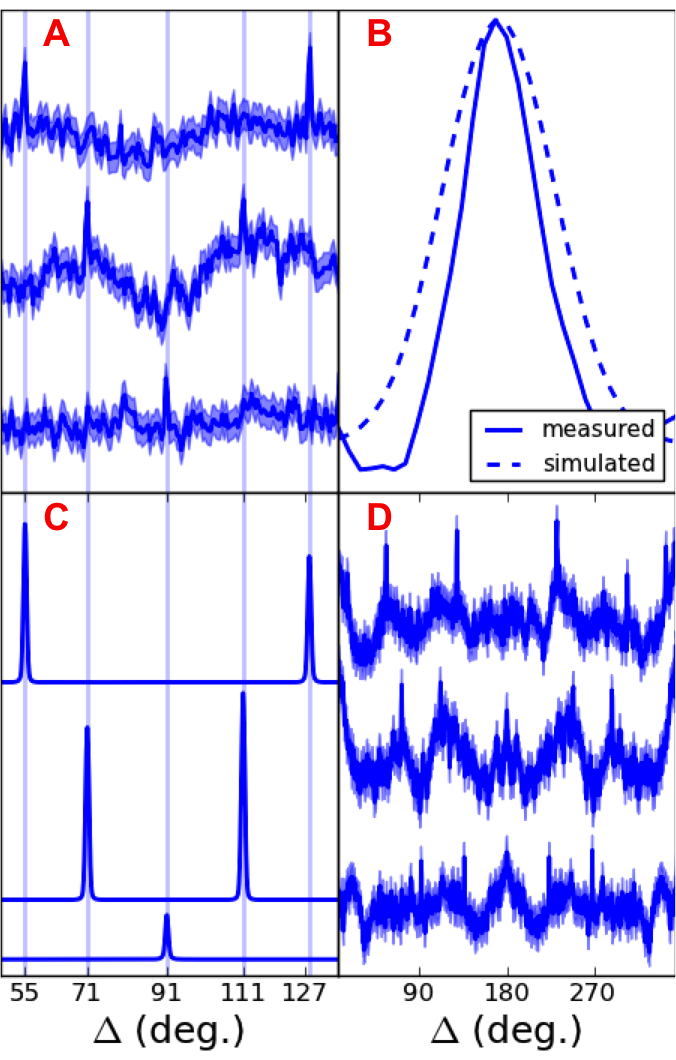
\includegraphics[ ]{../figures/royal_soc_figure_1.png}
\end{center}
{\bf Figure 1} A) from top to bottom, measurements of $C (|\vec{q}_{111}|,|\vec{q}_{200}|, \Delta  )$, $C (|\vec{q}_{111}|,|\vec{q}_{111}|, \Delta  )$, and $C (|\vec{q}_{200}|,|\vec{q}_{200}|, \Delta  )$.  Vertical lines mark analytical predictions and shading represents 95\% confidence intervals.  B) overlay of two correlations peaks from A and C. The width of the correlation peak is inversely proportional to the NP size, hence we conclude that the majority of our CXS signal resulted from scattering off of particles larger than 20 nm. C) from top to bottom, 20 nm silver NP simulations of $C (|\vec{q}_{111}|,|\vec{q}_{200}|, \Delta  )$, $C (|\vec{q}_{111}|,|\vec{q}_{111}|, \Delta  )$, and $C (|\vec{q}_{200}|,|\vec{q}_{200}|, \Delta  )$ D) same as A) but on the interval ($0-2\pi$ ). Despite application of a binary filter,  false correlations still arise due to systematic noises. Further refinement of the data is an ongoing process.
\end{figure}

Here we report on our attempts to resolve (\ref{angular}) at the two brightest silver Bragg rings. Specifically, we calculated $C (|\vec{q}_{111}|,|\vec{q}_{111}|, \Delta  )$, $C (|\vec{q}_{200}|,|\vec{q}_{200}|, \Delta  )$, and $C (|\vec{q}_{111}|,|\vec{q}_{200}|, \Delta  )$. 

Initial attempts to see convergence of the CXS signal were unsuccessful. In addition to the inherent statistical noises described in [1,7], CXS measurement  is very sensitive to systematic noises associated with the experimental conditions \cite{Kam:1981ua}, e.g. detector artifacts. The Pilatus 6M detector is made up of 60 pixel modules separated by 1-2 mm gaps, and each Bragg ring subtends multiple modules. The overall electronic response of each module is slightly different, causing false intensity correlations to dominate any underlying CXS. 

In order to minimize these parasitic correlations, we applied a binary filter to the data. We defined the filter as follows: Let $\{ \vec{q}_{hkl} \}_{m}$ represent the set of Bragg pixels on detector module $m$ where $1 \leq m \leq 60$. Let $\mu_m$ and $\sigma_m$ represent the average and standard deviation of $n_{s}(\vec{q})$  for all $\vec{q} \in \{ \vec{q}_{hkl} \}_{m} $ , respectively. Then for each $\vec{q} \in \{ \vec{q}_{hkl} \}_{m} $, we apply the photon count filter:

\[  n_{s}(\vec{q} ) = 
 \begin{cases} 
   1 & \quad \text{if } n_{s}(\vec{q} ) > \mu_m +  \sigma_m\\
   0 & \quad \text{otherwise} 
 \end{cases} 
 \]

i.e. all pixels less than one standard deviation above the mean are set to zero and the rest are set to unity. Hence, we only looked for correlations from the strongest Bragg peaks in each shot. Furthermore, the filter placed each detector module on the same scale, removing correlations between modules. [  will explain why 1 sigma was chosen here, after running some tests]  After applying the filter and calculating (\ref{angular}), the resulting correlations averaged to display peaks corresponding to the double Bragg scattering discussed above ( Figure 2 ). Despite the filtering, some artificial correlations persisted. We have discovered that the response of pixels within a module can also vary spatially, biasing the binary filter selection within the module and leading to artificial correlations. The low-order oscillations seen in Figure 2-A,D are most likely generated from such artifacts, as intra-module pixel response variation is relatively weak. Refinement of the data analysis is an ongoing process.

As mentioned above, we believe that the majority of our sample consisted of $10^9$ 20 nm silver NPs. From tabulated coherent atomic cross sections [ cite?] we estimated that each 20nm silver NP scattered roughly 1.6 photons per 0.7 sec exposure. We can further estimate that roughly 8.3\% of these NPs scatter into the Bragg ring at $q_{111}$ on the detector. (This is done by tracing out volumes of rotation of the reciprocal lattice points whose diameter is given by the Scherrer equation [8], and then determining which fraction of that volume intersects the Ewald sphere). These estimates are in line with the average photon counts per pixel per snapshot that we observed in the $q_{111}$ Bragg ring, $\approx$4 $10^4$. Many of the snapshots had Bragg peaks with counts $\approx$8 $10^8$, much greater than one would expect given standard Poisson photon statistics. Thus we conclude that our sample consisted of larger particles which scatter more photons. To put a lower bound on the size of these particles we again turn to the Scherrer equation, this time relating the width of the correlation peak to the particle size ( Figure 2-B ). We simulated (\ref{angular}) for 20 nm NPs and compared the width of a simulated correlation peak to the width of the corresponding measured one. We concluded that the correlations we are measuring are most likely generated by scattering off of thousands of $\approx$50 nm particles. We would like to emphasize that this is an estimated lower bound, for example thermal vibrations might cause a Bragg peak of a very large particle to broaden. It is one of our prime assumptions, however, that the particles remain roughly fixed throughout the exposure. Using volumetric arguments mentioned above  [REMOVE? for the estimating fraction of NP orientations which scatter into Bragg rings REMOVE ? ] , we estimated that roughly 0.5\% [ rough estimate, I'll put a number on it tomorrow] of 50 nm silver NP orientations will simultaneously subtend 2 Bragg peaks on the detector at either $q_{111}$ or $q_{200}$.

With the result of our measurement, we show that the theoretical Poisson noise [7] is not limiting the convergence of (\ref{converge}) in our simple case. We conclude that the main impediment to accurate measurements of CXS arises from systemic errors resulting from anisotropy artifacts induced by the detector system, which we have been able to partially overcome by the nonlinear filtering to a binary signal.

\section{Discussion}

Kam's original results \cite{Kam:1977wc} show that (\ref{correlation}), which may be directly calculated from the structure factors of the particle (\ref{structurefactor}) , may be derived from measurement of an ensemble of particles as a whole. Hence accurate measurement of CXS in the 3-dimensional $\{|\vec{q}_1|,|\vec{q}_2|,\Delta\}$ space can lead to constraints which can be placed on the electron density in a model, thus giving a route to iterative refinement (ref Brunger). 

Our results show that it is possible to obtain atomic scale information on the internal structure of a particle, from a bulk sample containing many identical  but randomly oriented particles, for the simple case of a silver NP. These results suggest that it should be feasible to obtain more detailed atomic scale constraints on models of more complex biomolecules by measuring scattering using pulses from x-ray free electron lasers (refs Hajdu, Chapman - Spence), provided one can effectively correct for experimentally induced sources of noise, particularly detector-induced correlations.

\section{D-References}

[1] Kam Z 1977 Determination of macromolecular structure in solution by spatial correlation of scattering fluctuations. Macromolecules 10 927-34

[2] Saldin D K, Poon H C, Bogan M J, Marchesini S, Shapiro D A, Kirian R A, Weierstall U and Spence J C H 2011 New light on disordered ensembles: ab initio structure determination of one particle from scattering fluctuations of many copies, Phys. Rev. Lett. 106 115501

[3] Kam Z, Koch M H J, and Bordas J 1981 Fluctuation x-ray-scattering from biological particles in frozen solution by using synchrotron radiation. Proc. Natl. Acad. Sci. USA 78 3559-62

[4] Wochner P, Gutt C, Autenrieth T, Demmer T, Bugaev V, Ortiz A D, Duri A, Zontone F, Grubel G and Dosch H 2009 X-ray cross correlation analysis uncovers hidden local symmetries in disordered matter. Proc. Natl Acad. Sci. USA 106 11511-4

[5] Kam Z and Gafni I 1985 3-dimensional reconstruction of the shape of human wart virus using spatial correlations. Ultramicroscopy 17 251�62

[6] Starodub D \textit{et al.} 2010 Single-particle structure determination by correlations of snapshot x-ray diffraction patterns. Nature Communications 3. (DOI: 10.1038/ncomms2288)

[7] Kirian R A, Schmidt K E, Wang X,  Doak R B , and Spence J C H  2011 Signal, noise, and resolution in correlated fluctuations from snapshot small-angle x-ray scattering.  Phys. Rev. E 84 011921

[8] Patterson A 1939  The Scherrer Formula for X-Ray Particle Size Determination. Phys. Rev. Vol56 10 978�982

% TJL to Dermen:
% You gotta learn to use bibtex/linked references. You're life will be *much* better in the long run!
% my citations look crazy b/c they are auto-generated
% Dermen to tjlane: I added some more refs.. can you add them to your auto gen list

\bibliographystyle{plain}
\begin{thebibliography}{1}

\bibitem{Kam:1977wc}
Z~Kam.
\newblock {Determination of macromolecular structure in solution by spatial
  correlation of scattering fluctuations}.
\newblock {\em Macromolecules}, 10(5):927--934, 1977.

\bibitem{Kam:1985tz}
Z~Kam and I~Gafni.
\newblock {Three-dimensional reconstruction of the shape of human wart virus
  using spatial correlations.}
\newblock {\em Ultramicroscopy}, 17(3):251--262, 1985.

\bibitem{Kam:1981ua}
Z~Kam, M~H Koch, and J~Bordas.
\newblock {Fluctuation x-ray scattering from biological particles in frozen
  solution by using synchrotron radiation.}
\newblock {\em Proceedings of the National Academy of Sciences},
  78(6):3559--3562, June 1981.

\bibitem{Saldin:2011ch}
D~Saldin, H~Poon, M~Bogan, S~Marchesini, D~Shapiro, R~Kirian, U~Weierstall, and
  J~Spence.
\newblock {New Light on Disordered Ensembles: Ab Initio Structure Determination
  of One Particle from Scattering Fluctuations of Many Copies}.
\newblock {\em Phys. Rev. Lett.}, 106(11):115501, March 2011.

\bibitem{Starodub:1fy}
D~Starodub, A~Aquila, S~Bajt, M~Barthelmess, A~Barty, C~Bostedt, J~D Bozek,
  N~Coppola, R~B Doak, S~W Epp, B~Erk, L~Foucar, L~Gumprecht, C~Y Hampton,
  A~Hartmann, R~Hartmann, P~Holl, S~Kassemeyer, N~Kimmel, H~Laksmono, M~Liang,
  N~D Loh, L~Lomb, A~V Martin, K~Nass, C~Reich, D~Rolles, B~Rudek, A~Rudenko,
  J~Schulz, R~L Shoeman, R~G Sierra, H~Soltau, J~Steinbrener, F~Stellato,
  S~Stern, G~Weidenspointner, M~Frank, J~Ullrich, L~Str~uuml der,
  I~Schlichting, H~N Chapman, J~C~H Spence, and M~J Bogan.
\newblock {Single-particle structure determination by correlations of snapshot
  X-ray diffraction patterns}.
\newblock {\em Nature Communications}, 3:1276--7, 1.

\bibitem{Wochner:2009ia}
Peter Wochner, Christian Gutt, Tina Autenrieth, Thomas Demmer, Volodymyr
  Bugaev, Alejandro~D{\'\i}az Ortiz, Agn{\`e}s Duri, Federico Zontone, Gerhard
  Gr{\"u}bel, and Helmut Dosch.
\newblock {X-ray cross correlation analysis uncovers hidden local symmetries in
  disordered matter.}
\newblock {\em P Natl Acad Sci Usa}, 106(28):11511--11514, July 2009.

\end{thebibliography}



\end{document}






